\section{Example for Slip on a 2D Subduction Zone}
\label{sec:example:subduction:2d}

PyLith features discussed in this example:
\begin{itemize}
\item Static solution
\item Quasi-static solution
\item CUBIT/Trelis mesh generation w/APREPRO
\item Nonplanar geometry
\item Variable mesh resolution
\item Linear triangular cells
\item HDF5 output
\item Dirichlet displacement and velocity boundary conditions
\item ZeroDispDB spatial database
\item UniformDB spatial database
\item SimpleDB spatial database
\item SimpleGridDB
\item Multiple materials
\item Nonlinear solver
\item Plane strain linearly elastic material
\item Plane strain linear Maxwell viscoelastic material
\item Prescribed slip
\item Spontaneous rupture
\item Multiple faults
\item Spatially variable coseismic slip
\item Spatially variable aseismic creep
\item Afterslip via fault friction
\item Static friction
\item Slip-weakening friction
\item Rate-state friction
\end{itemize}
All of the files necessary to run the examples are contained in the
directory \filename{examples/2d/subduction}.


\subsection{Overview}

This example examines quasi-static interseismic and coseismic
deformation in 2D for a subduction zone (see Figure
\vref{fig:example:subduction:2d:overview}).  It is based on the 2011
M9.0 Tohoku earthquake off the east coast of Japan. Figure
\vref{fig:example:subduction:2d:steps} shows the three steps of
increasing complexity. Step 1 focuses on the coseismic slip, Step 2
focuses on interseismic deformation, and Step 3 combines the two into
a pseudo-earthquake cycle deformation simulation. Step 4 focuses on
using the change in tractions from Step 1 to construct a simulation
with afterslip controlled by frictional sliding. Steps 5 and 6 replace
the prescribed aseismic slip on the subducting slab in Step 2 with a
frictional interface, producing spontaneous earthquake ruptures and
creep.

\begin{figure}
  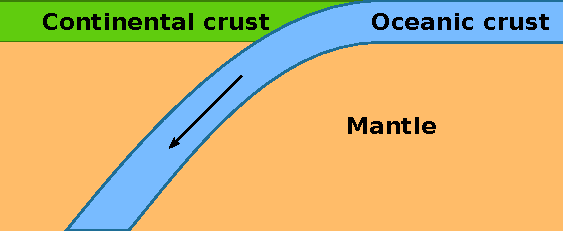
\includegraphics{examples/figs/subduction2d_cartoon_general}
  \caption{Cartoon of subduction zone example.}
  \label{fig:example:subduction:2d:overview}
\end{figure}

\begin{figure}
  \begin{tabular}{ccc}
    Step 1 & Step 2 & Step 3 \\
    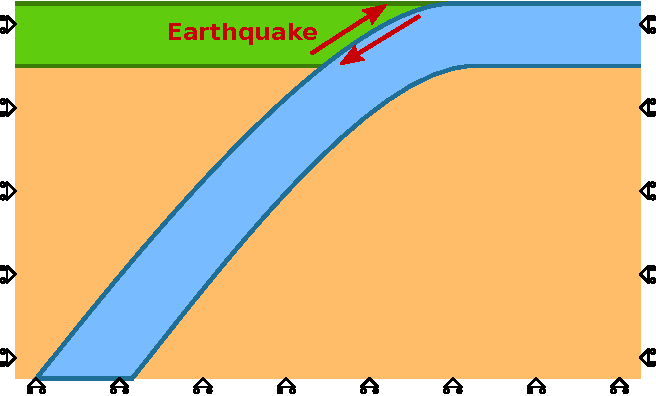
\includegraphics[width=2in]{examples/figs/subduction2d_step01} &
    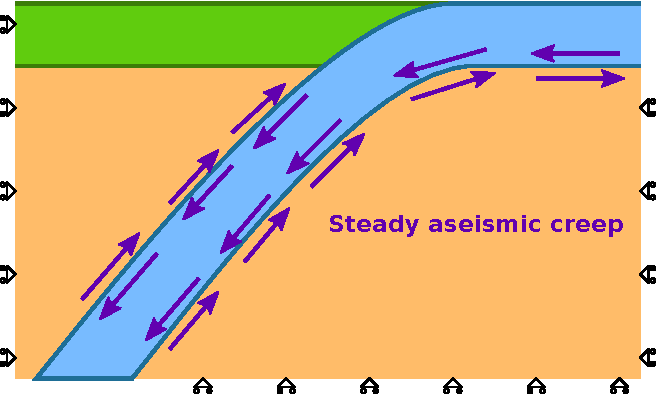
\includegraphics[width=2in]{examples/figs/subduction2d_step02} & 
    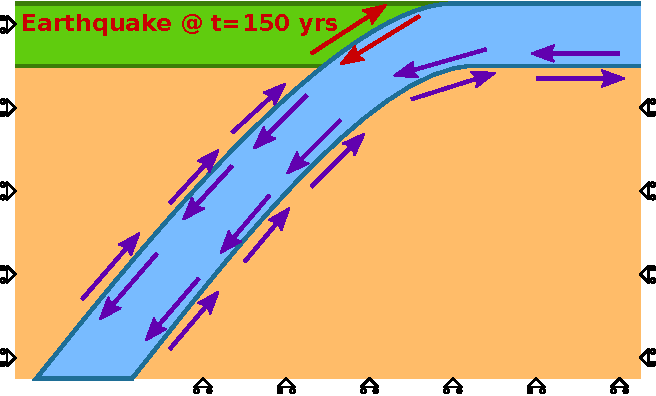
\includegraphics[width=2in]{examples/figs/subduction2d_step03} \\
  \end{tabular}
  \caption{Diagram of fault slip and boundary conditions for each step in the
    subduction zone example.}
  \label{fig:example:subduction:2d:steps}
\end{figure}


\subsection{Mesh Description}

We construct the mesh in CUBIT by constructing the geometry, prescribing
the discretization, running the mesher, and then grouping cells and
vertices for boundary conditions and materials. We use the APREPRO
programming language within the journal files to enable use of units
and to set variables for values used many times. An appendix in the
CUBIT documentation discusses the features available with APREPRO
in CUBIT. The CUBIT commands are in three separate journal files.
The main driver is in the journal file \filename{mesh\_tri3.jou}. It
calls the journal file \filename{geometry.jou} to construct the geometry
and \filename{createbc.jou} to set up the groups associated with boundary
conditions and materials. The journal files are documented and describe
the various steps outlined below.
\begin{enumerate}
\item Create the geometry defining the domain.
  \begin{enumerate}
  \item Create points.
  \item Connect points into spline curves.
  \item Split curves to separate them into sections bounding surfaces. 
  \item Connect curves into surfaces.
  \item Stitch surfaces together.
  \end{enumerate}
\item Define meshing scheme and cell size variation.
  \begin{enumerate}
  \item Define cell size along curves near fault.
  \item Increase cell size away from fault at a geometric rate (bias).
  \end{enumerate}
\item Generate mesh.
\item Create blocks for materials and nodesets for boundary conditions.
\item Export mesh.
\end{enumerate}

\begin{figure}
  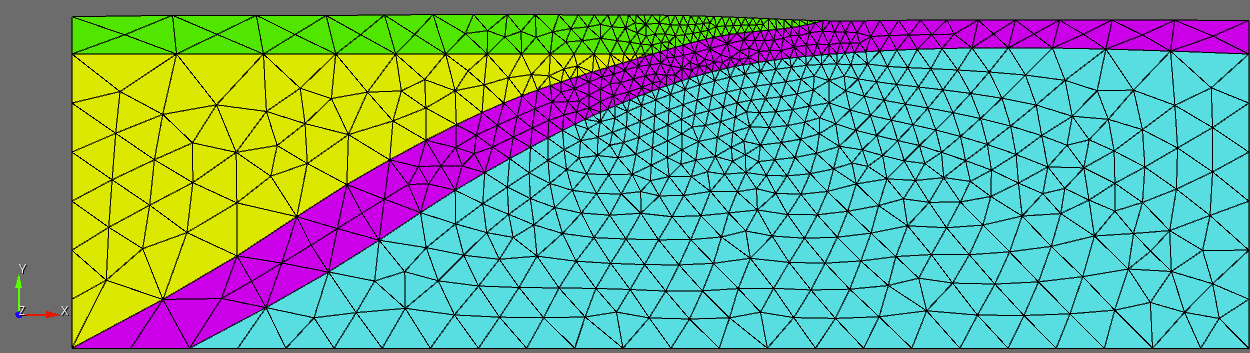
\includegraphics[width=4.5in]{examples/figs/subduction2d_tri3}
  \caption{Variable resolution finite-element mesh with triangular
    cells. The nominal cell size increases at a geometric rate of 1.2
    away from the region of coseismic slip.}
  \label{fig:example:subduction:2d:mesh}
\end{figure}


\subsection{Common Information}

As in the examples discussed in previous sections of these examples,
we place parameters common to the three steps in the \filename{pylithapp.cfg}
file so that we do not have to duplicate them for each step. The settings
contained in \filename{pylithapp.cfg} for this problem consist of:
\begin{inventory}
  \facilityitem{pylithapp.journal.info}{Settings that control the
    verbosity of the output written to stdout for the different
    components.}  \facilityitem{pylithapp.mesh\_generator}{Settings
    that control mesh importing, such as the importer type, the
    filename, and the spatial dimension of the mesh.}
  \facilityitem{pylithapp.timedependent}{Settings that control the
    problem, such as the total time, time-step size, and spatial
    dimension.}
  \facilityitem{pylithapp.timedependent.materials}{Settings that
    control the material type, specify which material IDs are to be
    associated with a particular material type, and give the name of
    the spatial database containing the physical properties for the
    material. The quadrature information is also given.}
  \facilityitem{pylithapp.problem.formulation.output}{Settings related
    output of the solution over the domain and subdomain (ground
    surface).}
  \facilityitem{pylithapp.timedependent.materials.\textit{MATERIAL}.output}{Settings
    related to output of the state variables for material
    \textit{MATERIAL}.}  \facilityitem{pylithapp.petsc}{PETSc settings
    to use for the problem, such as the preconditioner type.}
\end{inventory}
The physical properties for each material are specified in spatial
database files. For example, the elastic properties for the
continental crust are in \filename{mat\_concrust.spatialdb}. The
provided spatial database files all use just a single point to specify
uniform physical properties within each material. A good exercise is
to alter the spatial database files with the physical properties to
match PREM.


\subsection{Step 1: Coseismic Slip Simulation}

The first example problem is earthquake rupture involving coseismic
slip along the interface between the subducting slab and the continental
crust and uppermost portion of the mantle below the continental crust.
The spatial variation of slip comes from a cross-section of Gavin
Hayes' finite-source model \url{earthquake.usgs.gov/earthquakes/eqinthenews/2011/usc0001xgp/finite_fault.php}.
On the lateral and bottom boundaries of the domain, we fix the degrees
of freedom perpendicular to the boundary as shown in Figure \vref{fig:example:subduction:2d:steps}.
Parameter settings that augment those in \filename{pylithapp.cfg} are
contained in the file \filename{step01.cfg}. These settings are:
\begin{inventory}
  \facilityitem{pylithapp.timedependent.formulation.time\_step}{Adjust the total
    simulation time to 0 years (static simulation).}
  \facilityitem{pylithapp.timedependent}{Specifies the array of
    boundary conditions.}
  \facilityitem{pylithapp.timedependent.bc.\textit{BOUNDARY}}{Defines the settings
    for boundary \textit{BOUNDARY}, including which degrees of freedom
    are being constrained (x or y), the label (defined in\filename{ mesh\_tri3.exo})
    corresponding to the nodeset in CUBIT, and a label to the boundary
    condition used in any error messages.}
  \facilityitem{pylithapp.timedependent.interfaces.fault}{Specify the coseismic
    slip along the interface between the oceanic crust and continental
    crust with a small amount of slip penetrating into the upper mantle.}
  \facilityitem{pylithapp.problem.formulation.output.domain}{Gives the base filenames
    for HDF5 output (for example, \filename{step01.h5}).}
\end{inventory}
We run this example by typing
\begin{shell}
$ pylith step01.cfg
\end{shell}
The problem will produce twelve pairs of HDF5/Xdmf files. The HDF5
files contain the data and the Xdmf files contain the metadata required
by ParaView and Visit (and possibly other visualization tools that
use Xdmf files) to access the mesh and data sets in the HDF5 files.
The files include the solution over the domain and ground surface
(two pairs of files), physical properties, stress, and strain within
each material (eight pairs of files), and fault parameters, slip,
and traction (two pairs of files). 

Figure \vref{fig:example:subduction:2d:step01}, which was created using
ParaView, displays the magnitude of the displacement field with the
deformation exaggerated by a factor of 1000. 

\begin{figure}
  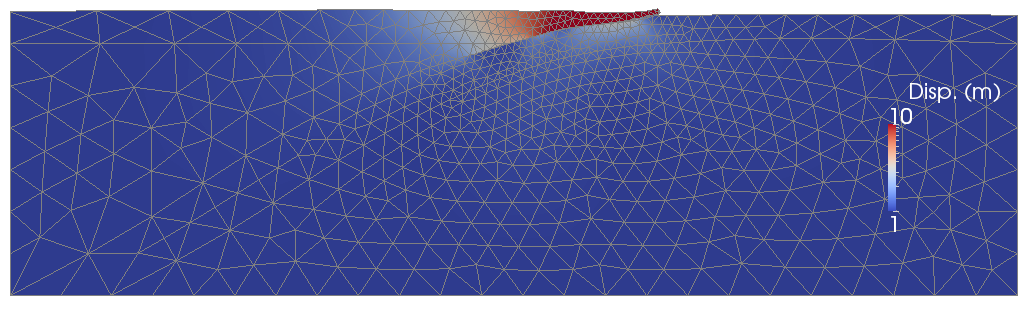
\includegraphics[width=4.5in]{examples/figs/subduction2d_step01_soln}
  \caption{Solution for Step 1. The colors indicate the magnitude of the displacement,
    and the deformation is exaggerated by a factor of 1000. }
  \label{fig:example:subduction:2d:step01}
\end{figure}


\subsection{Step 2: Interseismic Deformation Simulation}

In this example we simulate the interseismic deformation associated
with the oceanic crust subducting beneath the continental crust and
into the mantle. We prescribe steady aseismic slip of 8 cm/yr along
the interfaces between the oceanic crust and mantle with the interface
between the oceanic crust and continental crust locked as shown in
Figure \vref{fig:example:subduction:2d:steps}. We adjust the Dirichlet
boundary conditions on the lateral edges and bottom of the domain
by pinning only the portions of the boundaries in the mantle and continental
crust (i.e., not part of the oceanic crust). Parameter settings that
augment those in \filename{pylithapp.cfg} are contained in the file
\filename{step02.cfg}. These settings include:
\begin{inventory}
  \facilityitem{pylithapp.timedependent.formulation.time\_step}{Adjust the total
    simulation time to 100 years.}
  \facilityitem{pylithapp.timedependent}{Specifies the array of boundary conditions.}
  \facilityitem{pylithapp.timedependent.bc.\textit{BOUNDARY}}{Defines the settings
    for boundary \textit{BOUNDARY}, including which degrees of freedom
    are being constrained (x or y), the label (defined in\filename{ mesh\_tri3.exo})
    corresponding to the nodeset in CUBIT, and a label to the boundary
    condition used in any error messages.}
  \facilityitem{pylithapp.timedependent.interfaces}{Specify the steady aseismic
    slip as a constant slip rate on the fault surfaces.}
  \facilityitem{pylithapp.problem.formulation.output.domain}{Gives the base filename
    for HDF5 output (for example, \filename{step02.h5}).}
\end{inventory}
We run this example by typing
\begin{shell}
$ pylith step02.cfg
\end{shell}
The simulation will produce pairs of HDF5/Xdmf files with separate
files for each material and fault interface. Figure
\vref{fig:example:subduction:2d:step02}, which was created using
ParaView, displays the magnitude of the displacement field with the
deformation exaggerated by a factor of 1000. Using the animation
features within ParaView or Visit you can illustrate how the
continental crust near the trench subsides during the interseismic
deformation.

\begin{figure}
  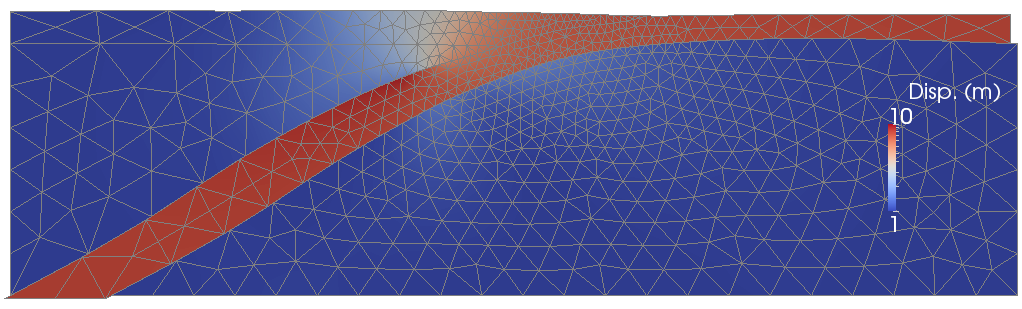
\includegraphics[width=4.5in]{examples/figs/subduction2d_step02_soln}
  \caption{Solution for Step 2 at 100 years. The colors indicate the
    magnitude of the displacement, and the deformation is exaggerated
    by a factor of 1000.}
  \label{fig:example:subduction:2d:step02}
\end{figure}


\subsection{Step 3: Pseudo-Earthquake Cycle Model}

This simulation combines 300 years of interseismic deformation from
Step 2 with the coseismic deformation from Step 1 applied at 150 years
to create a simple model of the earthquake cycle. Parameter settings
that augment those in \filename{pylithapp.cfg} are contained in the
file \filename{step03.cfg}. These settings include:
\begin{inventory}
  \facilityitem{pylithapp.timedependent.formulation.time\_step}{Adjust the total
    simulation time to 300 years.}
  \facilityitem{pylithapp.timedependent}{Specifies the array of boundary conditions.}
  \facilityitem{pylithapp.timedependent.bc.\textit{BOUNDARY}}{The Dirichlet boundary
    conditions match those in Step 2.}
  \facilityitem{pylithapp.timedependent.interfaces}{On the interface between the
    subducting oceanic crust and the mantle, we prescribe the same steady,
    aseismic slip as that in Step 2. On the interface along the top of
    the subducting oceanic crust and the continental crust and mantle
    we create two earthquake ruptures, The first rupture applies the coseismic
    slip form Step 1 at 150 years, while the second rupture prescribes
    the same steady, aseismic slip as in Step 2.}
  \facilityitem{pylithapp.problem.formulation.output.domain}{Gives the base filename
    for HDF5 output (for example, \filename{step03.h5}).}
\end{inventory}
We run this example by typing
\begin{shell}
$ pylith step03.cfg
\end{shell}
The simulation will produce pairs of HDF5/Xdmf files with separate
files for each material and fault interface. Figure \vref{fig:example:subduction:2d:step03},
which was created using ParaView, displays the magnitude of the displacement
field with the deformation exaggerated by a factor of 1000. Using
the animation features within ParaView or Visit you can illustrate
how the continental crust near the trench rebounds during the earthquake
after subsiding during the interseismic deformation. 

\begin{figure}
  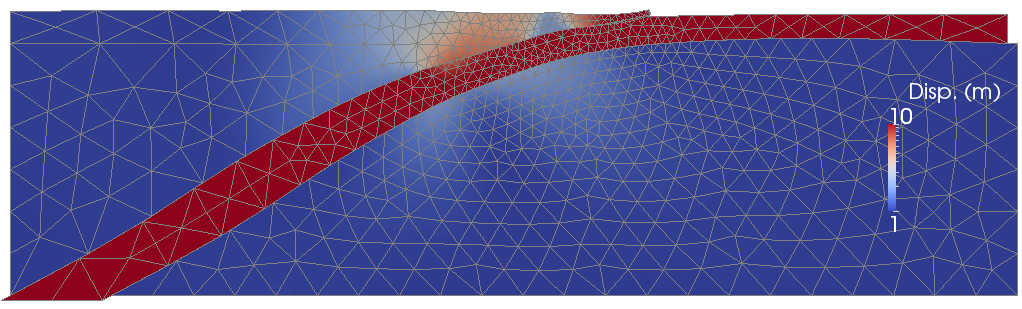
\includegraphics[width=4.5in]{examples/figs/subduction2d_step03_soln}
  \caption{Solution for Step 3 at 150 years (immediately following the earthquake
    rupture). The colors indicate the magnitude of the displacement, and
    the deformation is exaggerated by a factor of 1000.}
  \label{fig:example:subduction:2d:step03}
\end{figure}


\subsection{Step 4: Frictional Afterslip Simulation}

This simulation demonstrates how to combine the change in tractions
associated with coseismic slip with a background stress field to
compute afterslip controlled by static friction. The Python script
\filename{afterslip\_tractions.py} will create a spatial database file
with initial tractions based on the change in tractions from Step 1
and a background stress field.  The background stress field is simply
normal tractions consistent with the overburden (lithostatic load) for
a uniform half-space and shear tractions consistent with a coefficient
of friction of 0.6.  The \texttt{afterslip\_tractions.}  spatialdb
file is provided, so you do not need to run the Python script
\filename{afterslip\_tractions.py}; however, you can do so by typing
\begin{shell}
$ python afterslip_tractions.py
\end{shell}
We provide 2.0 MPa of strength excess associated with the background
stress field by using a cohesion of 2.0 MPa in the static friction
model. Slip will occur in regions where the coseismic slip increased
the shear tractions by more than 2.0 MPa. On the lateral and bottom
boundaries of the domain, we fix the degrees of freedom perpendicular
to the boundary as shown in Figure \vref{fig:example:subduction:2d:steps}.
Parameter settings that augment those in \filename{pylithapp.cfg} are
contained in the file \filename{step04.cfg}. These settings are:
\begin{inventory}
  \facilityitem{pylithapp.timedependent.formulation.time\_step}{Adjust the total
    simulation time to 0 years (static simulation).}
  \facilityitem{pylithapp.timedependent}{Selects the nonlinear solver and specifies
    the array of boundary conditions.}
  \facilityitem{pylithapp.timedependent.bc.\textit{BOUNDARY}}{Defines the settings
    for boundary \textit{BOUNDARY}, including which degrees of freedom
    are being constrained (x or y), the label (defined in\filename{ mesh\_tri3.exo})
    corresponding to the nodeset in CUBIT, and a label to the boundary
    condition used in any error messages.}
  \facilityitem{pylithapp.timedependent.interfaces.fault}{Specify a fault with
    a fault constitutive model (static friction) and initial fault tractions.}
  \facilityitem{pylithapp.problem.formulation.output.domain}{Gives the base filenames
    for HDF5 output (for example, \filename{step04.h5}).}
\end{inventory}

We run this example by typing
\begin{shell}
$ pylith step04.cfg
\end{shell}
The problem will produce twelve pairs of HDF5/Xdmf files. The HDF5
files contain the data and the Xdmf files contain the metadata required
by ParaView and Visit (and possibly other visualization tools that
use Xdmf files) to access the mesh and data sets in the HDF5 files.
The files include the solution over the domain and ground surface
(two pairs of files), physical properties, stress, and strain within
each material (eight pairs of files), and fault parameters, slip,
and traction (two pairs of files). 

Figure \vref{fig:example:subduction:2d:step04}, which was created using
ParaView, displays the magnitude of the displacement field with the
original configuration. Slip occurs down-dip from the coseismic slip
as well as in three areas with sharp gradients in slip, including
the trench. The location of the afterslip can be shifted by changing
the spatial variation of the coseismic slip and background stress
field.

\begin{figure}
  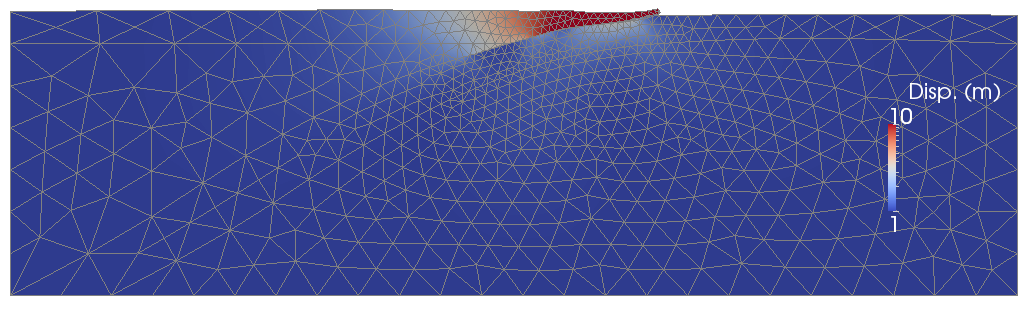
\includegraphics[width=4.5in]{examples/figs/subduction2d_step01_soln}
  \caption{Solution for Step 4. The colors indicate the magnitude of
    the displacement.}
  \label{fig:example:subduction:2d:step04}
\end{figure}


\subsection{Step 5: Spontaneous Earthquakes With Slip-Weakening Friction}

We simulate earthquake cycles over 100 years with spontaneous rupture
using slip-weakening friction. As in Step 4 including fault friction
requires the nonlinear solver. Through trial and error we choose a
time step of 2.5 years that permits reasonable convergence of the
nonlinear solver and runtime. 
\begin{cfg}
<h>[pylithapp.problem.formulation]</h>
# Fault friction is a nonlinear problem so we need to use the
# nonlinear solver.
<f>solver</f> = pylith.problems.SolverNonlinear

<h>[pylithapp.timedependent.formulation.time_step]</h>
<p>total_time</p> = 100.0*year
<p>dt</p> = 2.5*year
\end{cfg}
In simulations for research purposes, we
would use a higher resolution mesh and smaller time steps and
investigate the robustness of the solution to these parameters.

% Boundary conditions
We constrain the displacement normal to the lateral and bottom
boundaries without restraining the subducting slab. We also constrain
the vertical deformation of the west boundary to facilitate the
downward motion of the subducting slab.
\begin{cfg}
<h>[pylithapp.timedependent.bc.boundary_west]</h>
<p>bc_dof</p> = [0, 1]
<p>label</p> = bndry_west
<p>db_initial.label</p> = Dirichlet BC on west boundary
\end{cfg}

% Faults
We replace the prescribed aseismic slip
on the subduction interface that we used in Step 2 with a friction interface with the
slip-weakening fault constitutive model. 
\begin{cfg}
<h>[pylithapp.timedependent]</h>
<f>interfaces</f> = [fault_slabtop, fault_slabbot]

# Set the type of fault interface conditions.
<h>[pylithapp.timedependent.interfaces]</h>
<f>fault_slabtop</f> = pylith.faults.FaultCohesiveDyn
<f>fault_slabbot</f> = pylith.faults.FaultCohesiveKin
\end{cfg}

 % Fault - slab top
In order to generate stick-slip events, we need the coefficient of
friction to decrease with slip. We choose a slip-weakening friction
model with a dynamic coefficient of friction that is less than the
static coefficient of friction to provide this behavior. In
quasistatic modeling we use time steps much longer than the slip rise
time in an earthquake, so we want the slip confined to one time step
or just a few time steps. This means the drop in the coefficient of
friction should be independent in each time step; that is, we want the
fault to fully heal between time steps. This corresponds to setting
the \property{force\_healing} property of the \object{SlipWeakening}
object.

A common feature in numerical modeling of subduction zones is stable
sliding near the trench and below the seismogenic zone. We implement
stable sliding with the slip-weakening friction via a constant
coefficient of friction (equal values for the static and dynamic
coefficients of friction). We create a lower dynamic coefficient of
friction in the seismogenic zone, by introducing depth-dependent
variations in the dynamic coefficient of friction. using a
\object{SimpleGridDB} spatial database. As discussed in Section
\vref{sec:spatial:databases} This provides more efficient
interpolation compared to the \object{SimpleDB} implementation.
We impose initial tractions on the fault in a similar fashion as we
did in Step 4. We reduce the initial shear tractions slightly in the
seismogenic zone, consistent with a stress drop in the penultimate
earthquake followed by loading during the interseismic period.
\begin{cfg}
<h>[pylithapp.timedependent.interfaces.fault_slabtop]</h>
# --- Skipping general information discussed previously ---
# Friction
<f>friction</f> = pylith.friction.SlipWeakening
<p>friction.label</p> = Slip weakening
# Force healing after each time step, so weakening is confined to each
# time step and is not carried over into subsequent time steps.
<p>friction.force_healing</p> = True

<f>friction.db_properties</f> = spatialdata.spatialdb.SimpleGridDB
<p>friction.db_properties.label</p> = Slip weakening
<p>friction.db_properties.filename</p> = fault_slabtop_slipweakening.spatialdb

# Initial fault tractions
<f>traction_perturbation</f> = pylith.faults.TractPerturbation
<f>traction_perturbation.db_initial</f> = spatialdata.spatialdb.SimpleGridDB
<p>traction_perturbation.db_initial.label</p> = Initial fault tractions
<p>traction_perturbation.db_initial.filename</p> = fault_slabtop_tractions.spatialdb
\end{cfg}

% Solver
We adjust several of the solver tolerances. In general, we impose
larger tolerances to reduce runtime at the expense of a less accurate
solution. We set the zero tolerances for detecting slip and
suppressing fault opening to $1.0 \times 10^{-8}$. We want tolerances
for the linear solve to be smaller than these values, so we use an
absolute tolerance of $1.0 \times 10^{-9}$ and a very small relative
tolerance to force the residual below the absolute tolerance. We
impose an absolute tolerance for the nonlinear solver to be greater
than our zero tolerances and also force the residual to match the
absolute tolerance level by using a very small relative
tolerances. Finally, we set the parameters for the solver used to
calculate consistent values for the change in slip for a given change
in the Lagrange multipliers (which we sometimes call the friction
sensitivity solve).
\begin{cfg}
<h>[pylithapp.timedependent.interfaces.fault_slabtop]</h>
<p>zero_tolerance</p> = 1.0e-8
<p>zero_tolerance_normal</p> = 1.0e-8

# Convergence parameters.
<p>ksp_rtol</p> = 1.0e-20
<p>ksp_atol</p> = 1.0e-9
<p>ksp_max_it</p> = 1000

<p>snes_rtol</p> = 1.0e-20
<p>snes_atol</p> = 1.0e-7
<p>snes_max_it</p> = 1000

# Friction sensitivity solve used to compute the increment in slip
# associated with changes in the Lagrange multiplier imposed by the
# fault constitutive model.
<p>friction_pc_type</p> = asm
<p>friction_sub_pc_factor_shift_type</p> = nonzero
<p>friction_ksp_max_it</p> = 25
<p>friction_ksp_gmres_restart</p> = 30
<p>friction_ksp_error_if_not_converged</p> = true
\end{cfg}

We run this example by typing
\begin{shell}
$ pylith step05.cfg
\end{shell}
The problem will produce fourteen pairs of HDF5/Xdmf files. Figure
\vref{fig:example:subduction:2d:step05}, which was created using the
ParaView Python script \filename{viz/plot\_dispwarp.py} (see
Section~\vref{sec:ParaView:Python:scripts} for a discussion of how to
run ParaView Python scripts), displays the magnitude of the velocity
field with the original configuration exaggerated by a factor of
4000. Steady slip is largely confined to the stable sliding regions
with a sequence of ruptures in the seismogenic zone; most have a
duration of a few time steps, although most of the slip occurs in a
single time step. Figure~\ref{fig:example:subduction:2d:step05:slip}
shows the cumulative slip as a function of time and distance down dip
from the trench.

\begin{figure}
  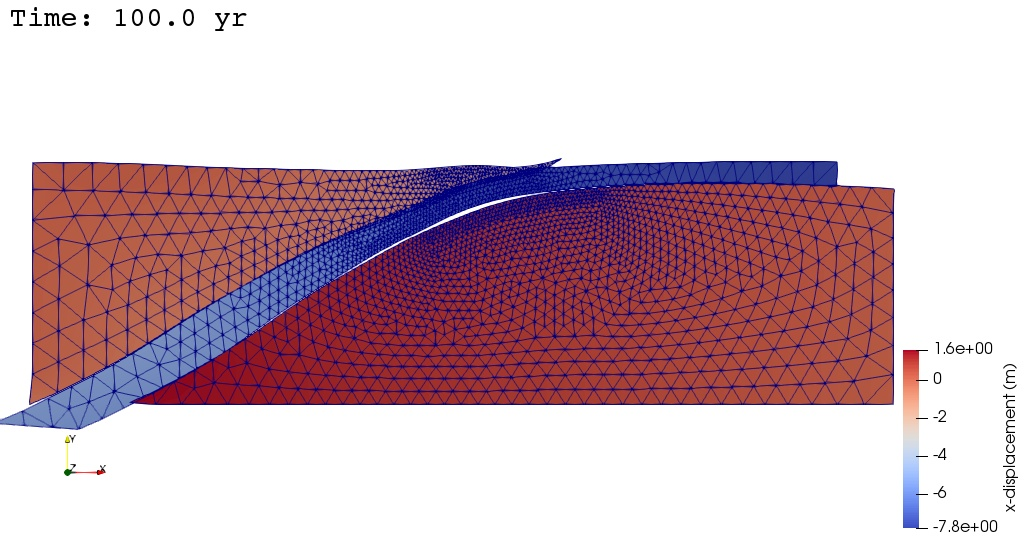
\includegraphics[width=4.5in]{examples/figs/subduction2d_step05_soln}
  \caption{Solution for Step 5 at the end of the simulation. The
    colors indicate the magnitude of the x-displacement component and
    the deformation has been exaggerated by a factor of 10,000. }
  \label{fig:example:subduction:2d:step05}
\end{figure}

\begin{figure}
  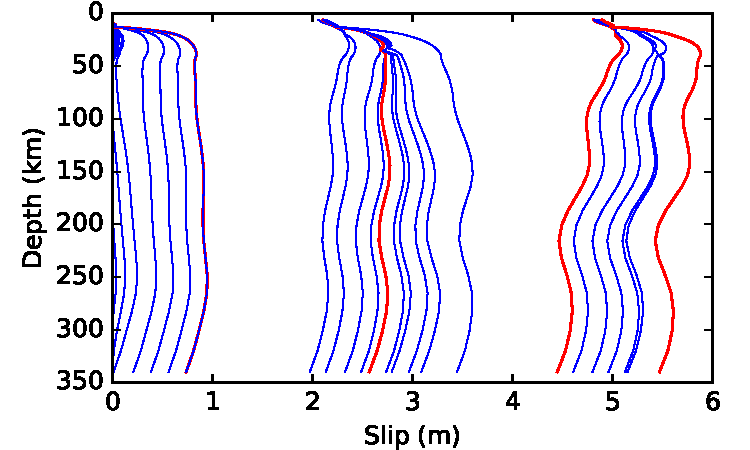
\includegraphics[width=4.5in]{examples/figs/subduction2d_step05_slip}
  \caption{Cumulative slip as a function of time and depth in Step
    5. The red lines indicate slip every 10 time steps.}
  \label{fig:example:subduction:2d:step05:slip}
\end{figure}


\subsection{Step 6: Spontaneous Earthquakes With Rate-State Friction}

In this example we replace the slip-weakening in Step 5 with rate- and
state-friction using the ageing law. We also lengthen the duration of
the simulation to 200 years and reduce the time step to 1.0 years,
which were determined through trial and error to get a couple
earthquake cycles with reasonable convergence for this relatively
coarse resolution mesh.
\begin{cfg}
<h>[pylithapp.timedependent.formulation.time_step]</h>
<p>total_time</p> = 200.0*year
<h>dt</h> = 1.0*year
\end{cfg}

The specification of the parameters for the rate- and state-friction
model follow a similar pattern to the ones for the slip-weakening
friction in Step 5. Our regularization of the coefficient of friction
for near zero slip rate values involves a transition to a linear
dependence on slip rate; in this example we specify that this
transition should occur at a nondimensional slip rate of
$1.0 \times 10^{-6}$. We impose depth variation of the friction model
parameters via a \object{SimpleGridDB} spatial database in order to
generate earthquake-like ruptures in the seismogenic zone with stable
sliding above and below. For the initial tractions, we impose uniform
values using a \object{SimpleDB} spatial database. We set the initial
state for the friction model to be roughly consistent with steady
state sliding at the reference coefficient of friction at the
reference slip rate, and include it in the state variable in the
output as a check.
\begin{cfg}
<h>[pylithapp.timedependent.interfaces.fault_slabtop]</h>
# --- Skipping parameters discussed in previous examples. ---
# Friction
<f>friction</f> = pylith.friction.RateStateAgeing
<p>friction.label</p> = Rate-state friction
# Nondimensional slip rate below which friction depends linearly on slip rate.
<p>friction.linear_slip_rate</p> = 1.0e-6

# Set spatial database for distribution of friction parameters
<f>friction.db_properties</f> = spatialdata.spatialdb.SimpleGridDB
<p>friction.db_properties.label</p> = Slip weakening
<p>friction.db_properties.filename</p> = fault_slabtop_ratestate.spatialdb

# Set spatial database for the initial value of the state variable.
<f>friction.db_initial_state</f> = spatialdata.spatialdb.UniformDB
<p>friction.db_initial_state.label</p> = Rate State Ageing State
<p>friction.db_initial_state.values</p> = [state-variable]
# theta_ss = characteristic_slip_dist / reference_slip_rate
<p>friction.db_initial_state.data</p> = [20.0*year]

# Initial fault tractions
<f>traction_perturbation</f> = pylith.faults.TractPerturbation
<f>traction_perturbation.db_initial</f> = spatialdata.spatialdb.UniformDB
<p>traction_perturbation.db_initial.label</p> = Initial fault tractions
<p>traction_perturbation.db_initial.values</p> = [traction-shear, traction-normal]
<p>traction_perturbation.db_initial.data</p> = [-12.0*MPa, -20.0*MPa]

<h>[pylithapp.problem.interfaces.fault_slabtop.output]</h>
<f>writer</f> = pylith.meshio.DataWriterHDF5
<p>writer.filename</p> = output/step06-fault-slabtop.h5
<p>vertex_info_fields</p> = [normal_dir, strike_dir]
<p>vertex_data_fields</p> = [slip, slip_rate, traction, state_variable]
\end{cfg}

We run this example by typing
\begin{shell}
$ pylith step06.cfg
\end{shell}
The problem will produce fourteen pairs of HDF5/Xdmf files. Figure
\vref{fig:example:subduction:2d:step06}, which was created using the
ParaView Python script \filename{viz/plot\_dispwarp.py}, displays the
magnitude of the velocity field with the original configuration
exaggerated by a factor of 4000. Steady slip is largely confined to
the stable sliding regions with a sequence of ruptures in the
seismogenic zone; note how the rate-state friction allows a more
natural nucleation of the ruptures compared to the slip-weakening
friction. Figure~\ref{fig:example:subduction:2d:step05:slip} shows the
cumulative slip as a function of time and distance down dip from the
trench.

\begin{figure}
  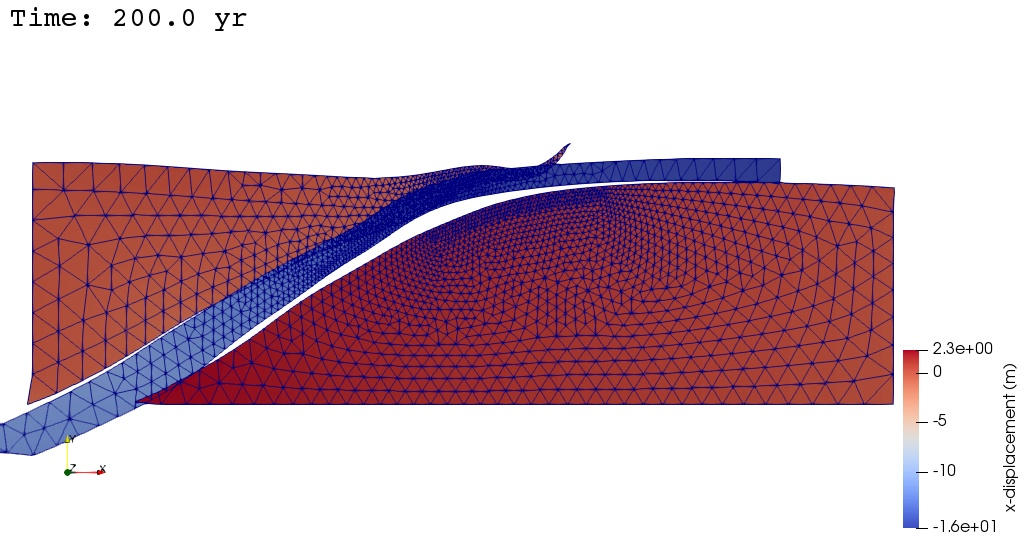
\includegraphics[width=4.5in]{examples/figs/subduction2d_step06_soln}
  \caption{Solution for Step 6 at the end of the simulation. The
    colors indicate the magnitude of the x-displacement component and
    the deformation has been exaggerated by a factor of 10,000.}
  \label{fig:example:subduction:2d:step06}
\end{figure}

\begin{figure}
  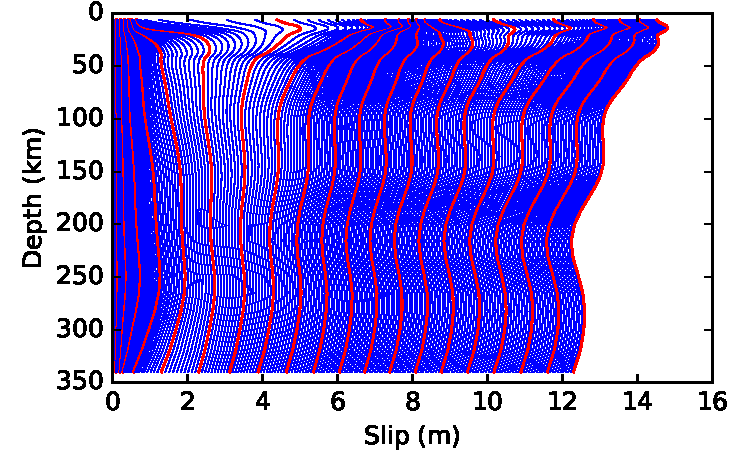
\includegraphics[width=4.5in]{examples/figs/subduction2d_step06_slip}
  \caption{Cumulative slip as a function of time and depth in Step
    6. The red lines indicate slip every 10 time steps.}
  \label{fig:example:subduction:2d:step06:slip}
\end{figure}


\subsection{Exercises}

The list below includes some suggested modifications to these examples
that will allow you to become more familiar with PyLith while
examining some interesting physics.
\begin{itemize}
\item Change the resolution of the mesh by editing the \filename{mesh\_tri3.jou}
  journal file. Change the resolution and bias factor.
\item Add depth dependent viscosity to the mantle and crust. This requires
  using the linear Maxwell plane strain bulk constitutive model in the
  crust as well and creating spatial databases that include viscosity
  for the crust. Specifying a depth dependent variation in the parameters
  will require adding points, updating num-locs accordingly, and changing
  data-dim to 1.
\item Modify the spatial database files for the material properties to use
  depth-dependent elastic properties based on PREM (Dziewonski and Anderson,
  1981, 10.1016/0031-9201(81)90046-7). See \url{geophysics.ou.edu/solid_earth/prem.html}
  for a simple table of values. Add points, update num-locs accordingly,
  and change data-dim to 1.
\item Modify the CUBIT journal files to use quad4 cells rather than tri3
  cells. This requires using the pave mesh scheme.
\item Modify Steps 5 and 6 to use a user-defined variable time
  step. Experiment with longer time steps between earthquake ruptures
  and smaller time steps around the time of the earthquake
  ruptures. Can you develop a simple algorithm for choosing the time step?
\item Adjust the parameters of the friction models and examine the
  effects on the deformation and the convergence of the nonlinear
  solve. In which cases do you need to adjust the time step to retain
  reasonable convergence?
\end{itemize}


% End of file
